% !TEX TS-program = pdflatex
% !TEX encoding = UTF-8 Unicode
% !TEX root = main.tex
% !TEX spellcheck = en-US
% ****************************************************************************************
% File: main.tex
% Author: Jakob Spindler
% Date: 2024-10-16
% ****************************************************************************************
\documentclass[a4paper,11pt,oneside,final,titlepage,openany,onecolumn]{report}
% input preamble (include additional packages, set options, define macros)
% !TEX TS-program = pdflatex
% !TEX encoding = UTF-8 Unicode
% !TEX root = ../main.tex
% !TEX spellcheck = en-US
% ****************************************************************************************
% File: _preamble.tex
% Author: Jakob Spindler
% Date: 2024-10-16
% ****************************************************************************************
% ****************************************************************************************
% General settings (input encoding, font encoding, font, language)
% ****************************************************************************************
\usepackage[utf8]{inputenc} % character encoding used in input file
\usepackage[T1]{fontenc} % specifies the encoding used in the fonts
\usepackage{lmodern} % provides more support for non-ASCII characters than cm-super
\usepackage{microtype} % improves line-filling when using PDFLaTeX
\usepackage[ngerman,english]{babel} %  last language is considered the main one
\renewcommand{\familydefault}{\sfdefault} % select a sans serif font family 

% \pdfsuppresswarningpagegroup=1 % suppress warning when including PDFs with page groups

% ****************************************************************************************
% Basic macros for thesis
% ****************************************************************************************
\newcommand{\authorName}{Jakob Spindler}
\newcommand{\authorContact}{sj0458@mci4me.at}

\newcommand{\department}{Department of Technology \& Life Sciences}
\newcommand{\docTitle}{PID Controller Design for a Buck Converter}
\newcommand{\docType}{Report}
\newcommand{\studyProgram}{Master's program Mechatronics \& Smart Technologies}
\newcommand{\degree}{Master of Science in Engineering}
\newcommand{\studyYear}{MA-MECH-23-VZ}
\newcommand{\supervisorName}{Thomas Gadner}
\newcommand{\supervisorContact}{}
\newcommand{\assesorName}{Dr. Georg Saxl}
\newcommand{\assesorContact}{georg.saxl@mci.edu}
\newcommand{\university}{Management Center Innsbruck}
\newcommand{\matnr}{11941482}


\newcommand{\authorAName}{Liam Nolan}
\newcommand{\authorAContact}{nl6496@mci4me.at}
\newcommand{\authorBName}{Johannes Schmid}
\newcommand{\authorBContact}{sj0751@mci4me.at}
\newcommand{\authorCName}{Jakob Spindler}
%\newcommand{\authorCContact}{sj0458@mci4me.at}
\newcommand{\courseName}{WS 2024 Transient Simulation }
\newcommand{\courseCode}{MECH-M-3-SVE-TSI-ILV
}
%\newcommand{\department}{Department of Technology \& Life Sciences}
%\newcommand{\docTitle}{Optimization Study of a flow heater}
%\newcommand{\docType}{Report}
%\newcommand{\studyProgram}{Master's program Mechatronics \& Smart Technologies}
%\newcommand{\studyYear}{MA-MECH-23-VZ}
\newcommand{\lecturerName}{Manuel Berger, PhD}
\newcommand{\lecturerContact}{manuel.berger@mci.edu}
%\newcommand{\university}{Management Center Innsbruck}
% Definition of BibTeX macro used in IEEEexample
\newcommand{\BibTeX}{BibTeX}

% ****************************************************************************************
% Drawing and plotting, scientific packages, 
% ****************************************************************************************
% For use of subfigure environment
\usepackage{subcaption}

% For use of cmidrule in table environment
\usepackage{booktabs}

\usepackage{makecell}

% Handling of images
\usepackage{graphicx}
\graphicspath{{./img/}}

% Colour support
\usepackage[table]{xcolor}

% Handling of MATLAB code
%\usepackage{mcode}

% Tabulars with adjustable-width columns
\usepackage{tabularx}
\usepackage{multirow}

% Sketching and importing MATLAB plots
\usepackage{pgfplots}
\usepackage{grffile}
\pgfplotsset{compat=newest}
\usetikzlibrary{plotmarks}
\usetikzlibrary{arrows.meta}
\usetikzlibrary{patterns}
\usepgfplotslibrary{patchplots}
\pgfplotsset{plot coordinates/math parser=false}
\newlength\figureheight
\newlength\figurewidth

% Typesetting electrical networks
\usepackage{circuitikz}

% scientific packages
\usepackage{amsmath}
\usepackage{amsfonts}
\usepackage{xfrac}
\usepackage{siunitx}
\AtBeginDocument{\sisetup{
		mode=match,
		unit-font-command = \mathrm,
		reset-text-family=false,
		reset-text-series=false,
		reset-text-shape=false,
		exponent-product=\cdot
	}}
\DeclareSIUnit\unity{1} % can be used for dimensionless quantities
\DeclareSIUnit\sample{Sa}
% ****************************************************************************************
% Referencing and citing
% ****************************************************************************************
% Caption settings
\usepackage[
	format=plain, % typeset as normal paragraph
	labelformat=simple, % typeset label as name and number
	labelsep=period, % caption label and text separated by period and space
	textformat=simple, % caption text typeset as is
	justification=justified, % typset caption as normal paragraph
	singlelinecheck=true, % automatically center short captions
	font=small,
	labelfont=bf, % set bold font for label
	width=.75\textwidth % set fixed width for caption
]{caption}
\captionsetup[table]{position=top}
\captionsetup[figure]{position=bottom}

% Hypertext marks (should be loaded last but before geometry)
\usepackage[hyperindex]{hyperref}
% Extension options
\hypersetup{
	colorlinks, % colours the text of links and anchors (instead of borders)
	linkcolor={blue!65!black},
	citecolor={blue!65!black},
	urlcolor={blue!65!black}
}
% PDF display and information options
\hypersetup{
	pdftitle={\docTitle},
	pdfsubject={\docType},
	pdfauthor={\authorName},
	pdfkeywords={},
	pdfcreator={pdflatex},
	pdfproducer={LaTeX with hyperref}
}

% formatting of cross-references
\usepackage[capitalise]{cleveref}
\crefformat{equation}{(#2#1#3)}
\Crefformat{equation}{Equation~(#2#1#3)}

%matlab prettifier
\usepackage{matlab-prettifier}

% ****************************************************************************************
% Bibliography settings
% ****************************************************************************************
% template from https://www.ieee.org/conferences/publishing/templates.html
\usepackage[
	backend=biber,
	style=numeric-comp, % numeric style with compact multiple citations i.e. [1-5] and not [1,2,3,4,5]
	natbib=true,
	sorting=none
]{biblatex}
%\addbibresource{zotero.bib}
\addbibresource{bib.bib}

% ****************************************************************************************
% Glossary (acronyms, list of symbols) settings
% ****************************************************************************************
\usepackage[acronym,nomain,nonumberlist,nopostdot,sort=def,toc]{glossaries}
\renewcommand*{\glstextformat}[1]{\textcolor{black}{#1}} % make links appear black
\newglossary[slg]{symbolslist}{syi}{syg}{List of Symbols} % define custom glossary
\glsaddkey% define custom key
	{unit}% key
	{\glsentrytext{\glslabel}}% default value
	{\glsentryunit}% command analogous to \glsentrytext
	{\GLsentryunit}% command analogous to \Glsentrytext
	{\glsunit}% command analogous to \glstext
	{\Glsunit}% command analogous to \Glstext
	{\GLSunit}% command analogous to \GLStext
\glssetnoexpandfield{unit}
\makeglossaries % create makeindex files

\newglossarystyle{symbolsliststyle}{%
	\setglossarystyle{long3col}% style based on long3col
	\renewenvironment{theglossary}{%
		\begin{longtable}{lp{\glsdescwidth}>{\arraybackslash}p{2cm}}}%
		{\end{longtable}}%
	\renewcommand*{\glossaryheader}{% change the table header
		\bfseries Symbol & \bfseries Description & \bfseries Unit\\\hline%
		\endhead}%
	\renewcommand*{\glossentry}[2]{% change the displayed items
		\glstarget{##1}{\glossentryname{##1}}% name
		& \glossentrydesc{##1}% description
		& $\glsentryunit{##1}$% unit
		\tabularnewline
	}%
}

% ****************************************************************************************
% Page layout and headers
% ****************************************************************************************
% Specify page layout (paper name and orientation specified in document class options)
\usepackage[
	includeheadfoot, % includes the head of the page into total body
	ignoremp, % disregards marginal notes in determining the horizontal margins
	nomarginpar, % shrinks spaces for marginal notes to 0pt
	hmargin=1.5in, % left and right margin
	vmargin=1in, % top and bottom margin
	headheight=14pt %  height of header
]{geometry}

\usepackage{parskip} % helps in implementing paragraph layouts

% Header and footer settings
\usepackage{fancyhdr}
\pagestyle{fancy} % set page style to 'fancy'
\renewcommand{\chaptermark}[1]{\markboth{\thechapter.\ #1}{}}
% \renewcommand{\sectionmark}[1]{\markright{\thesection.\ #1}}
\fancyhf{} % clear all header and footer fields
\fancyhead[L]{\leftmark} % set left header location (chapter)
% \fancyhead[R]{\rightmark} % set right header location (section)
\fancyfoot[C]{\thepage} % set center footer location (page count)

% ****************************************************************************************
% Packages for testing purposes (can be deleted)
% ****************************************************************************************
\usepackage{lipsum}
\usepackage{blindtext}
\usepackage{todonotes}
%\usepackage{superscript}

% EOF
\loadglsentries{./tex/_/_defns.tex}
\makeglossaries
\begin{document}
	\pagenumbering{alph}
	% !TEX TS-program = pdflatex
% !TEX encoding = UTF-8 Unicode
% !TEX root = ../main.tex
% !TEX spellcheck = en-US
% ****************************************************************************************
% File: titlepage.tex
% Author: Jakob Spindler
% Date: 2024-10-16
% ****************************************************************************************

\thispagestyle{empty}
\pdfbookmark[0]{Title page}{titlepage} % sets a PDF bookmark
\thispdfpagelabel{} %  set page number shown in the tool bar of a PDF viewer
\begin{center}
	\textbf{\Huge \university}\par
	\vspace{8ex}\par
	\textbf{\LARGE \department}\par
	\vspace{4ex}\par
	\textbf{\Large \studyProgram}\par
	\vspace{4ex}\par
	
\includegraphics[scale = 0.75]{MCI_Logo.pdf}\par
	\vspace{4ex}\par
	\textbf{\LARGE \docType}\par
	\vspace{2ex}\par
	\textbf{composed as part of the course\\[0.5ex] \courseName{} (\courseCode)}\par
	\vspace{4ex}\par
	\textbf{about}\par
	\vspace{4ex}\par
	\textbf{\LARGE \docTitle}\par
	\vspace{4ex}\par
	\textbf{from}\par
	\vspace{4ex}\par
	\textbf{\Large \href{\authorContact}{\authorName}}
\end{center}
\vspace{4ex}
\begin{tabular}{ll}
	Study program & \studyProgram\\[0.5ex]
	Year & \studyYear\\[0.5ex]
	Course & \courseName{} (\courseCode)\\[0.5ex]
	Name of supervisor & \href{\lecturerContact}{\supervisorName}\\[0.5ex]
	Submission deadline & January 27, 2024
\end{tabular}
\vfill
\begin{center}
	\today
\end{center}
%EOF
	\pagenumbering{Roman}
	\pdfbookmark[0]{\contentsname}{toc} % sets a PDF bookmark
 
    \tableofcontents
	\newcounter{romanpagecount}
	\setcounter{romanpagecount}{\value{page}}
	\clearpage
	\pagenumbering{arabic}

	% add content here
    
    

	% !TEX TS-program = pdflatex
% !TEX encoding = UTF-8 Unicode
% !TEX root = ../main.tex
% !TEX spellcheck = en-US
% ****************************************************************************************
% File: introduction.tex
% Author: Jakob Spindler
% Date: 2024-10-16
% ****************************************************************************************
\chapter{Introduction}
\label{chapter:introduction}

A discrete \gls{acr:pid} controller for a \qty{12}{\volt} to \qty{5}{\volt} Buck-Converter is to be designed and tested using PLECS \autocite{PLECSPlexim}.

The passive components of the Buck-Converter are chosen as :

\begin{table}[htbp]
    \centering
    \begin{tabular}{c|c}
        Component & Value \\ \hline
        $L$ & \qty{20}{\micro\henry} \\ 
        $C$ & \qty{50}{\micro\farad} \\ 
        $R$ & \qty{5}{\ohm} \\ 
    \end{tabular}
    \caption{Passive components of the Buck-Converter}
    \label{tab:components}
\end{table}

A continous controller can be designed according to \autocite{samosirSimpleFormulaDesigning2023} and thus yields:

\begin{table}[htbp]
    \centering
    \begin{tabular}{c|c}
        Parameter & Value \\ \hline
        $K_D$ & $50 LC$ \\ 
        $K_P$ & $50 \frac{L}{R}$ \\ 
        $K_I$ & $50$ \\ 
    \end{tabular}
    \caption{Initial PID Controller Parameters}
    \label{tab:pid_parameters}
\end{table}

The parameters were adjusted imperically for a sampling time of \qty{1}{\milli\second} to yield a stable and fast responding system and can be found in \autoref{tab:final_pid_parameters}.

\begin{table}[htbp]
    \centering
    \begin{tabular}{c|c}
        Parameter & Value \\ \hline
        $K_D$ & $50 LC$ \\ 
        $K_P$ & $\frac{L}{R}$ \\ 
        $K_I$ & $20$ \\ 
    \end{tabular}
    \caption{Final PID Controller Parameters}
    \label{tab:final_pid_parameters}
\end{table}




% EOF
	% !TEX TS-program = pdflatex
% !TEX encoding = UTF-8 Unicode
% !TEX root = ../main.tex
% !TEX spellcheck = en-US
% ****************************************************************************************
% File: methods.tex
% Author: Jakob Spindler
% Date: 2024-10-16
% ****************************************************************************************
\chapter{Methods}
\label{chapter:methods}

The PLECS model of the converter includes the following:
\begin{itemize}
    \item a PID controlled duty cycle
    \item a noise source for the input voltage
    \item a variable load
\end{itemize}

all of which can be selected to be active or inactive as can be seen in \autoref{fig:PLECS_model} and \autoref{fig:PLECS_subsystems}.

\begin{figure}[htbp]
    \centering
    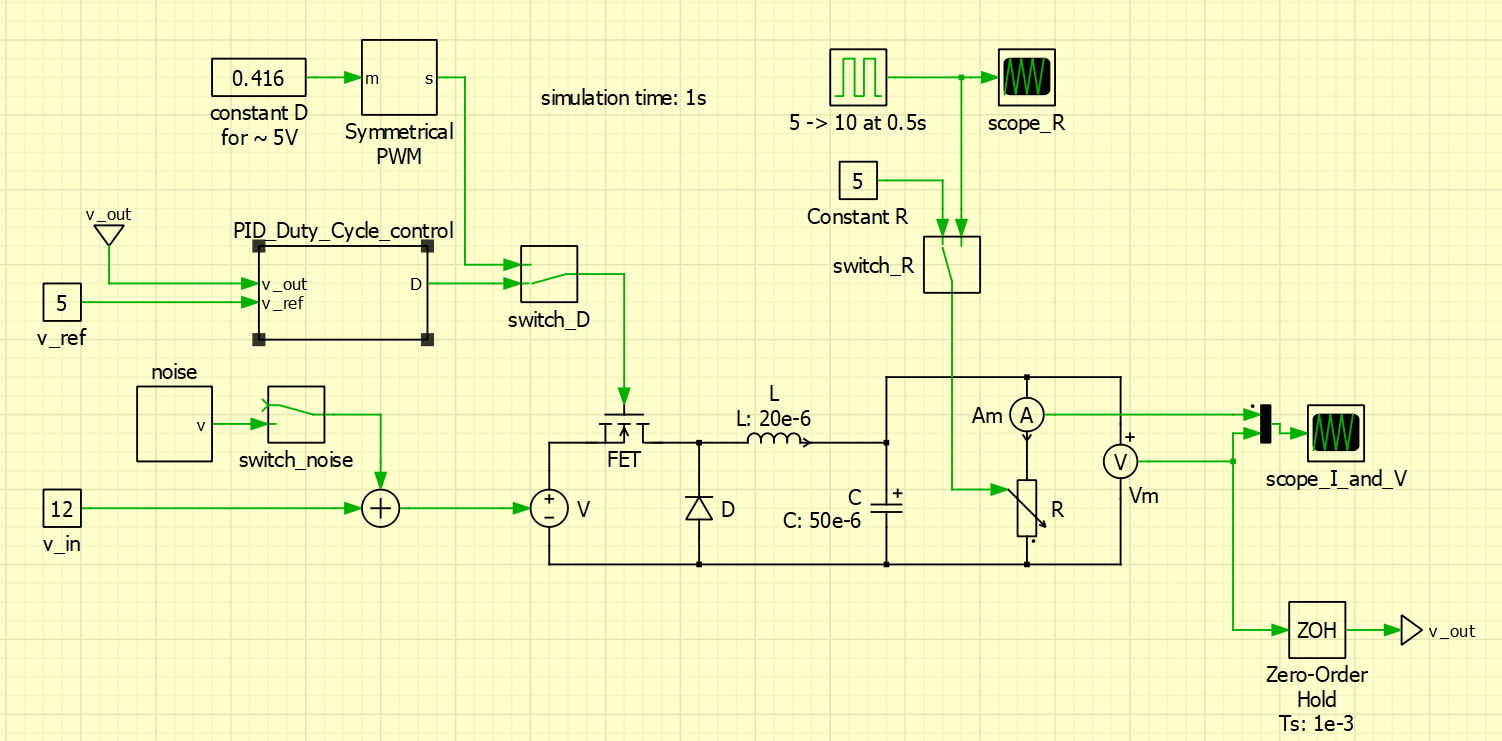
\includegraphics[width=1\textwidth]{img/PLECS_model_full_view.png}
    \caption{PLECS model of the Buck-Converter}
    \label{fig:PLECS_model}
\end{figure}

\begin{figure}[htbp]
    \centering
    \begin{subfigure}[b]{0.55\textwidth}
        \centering
        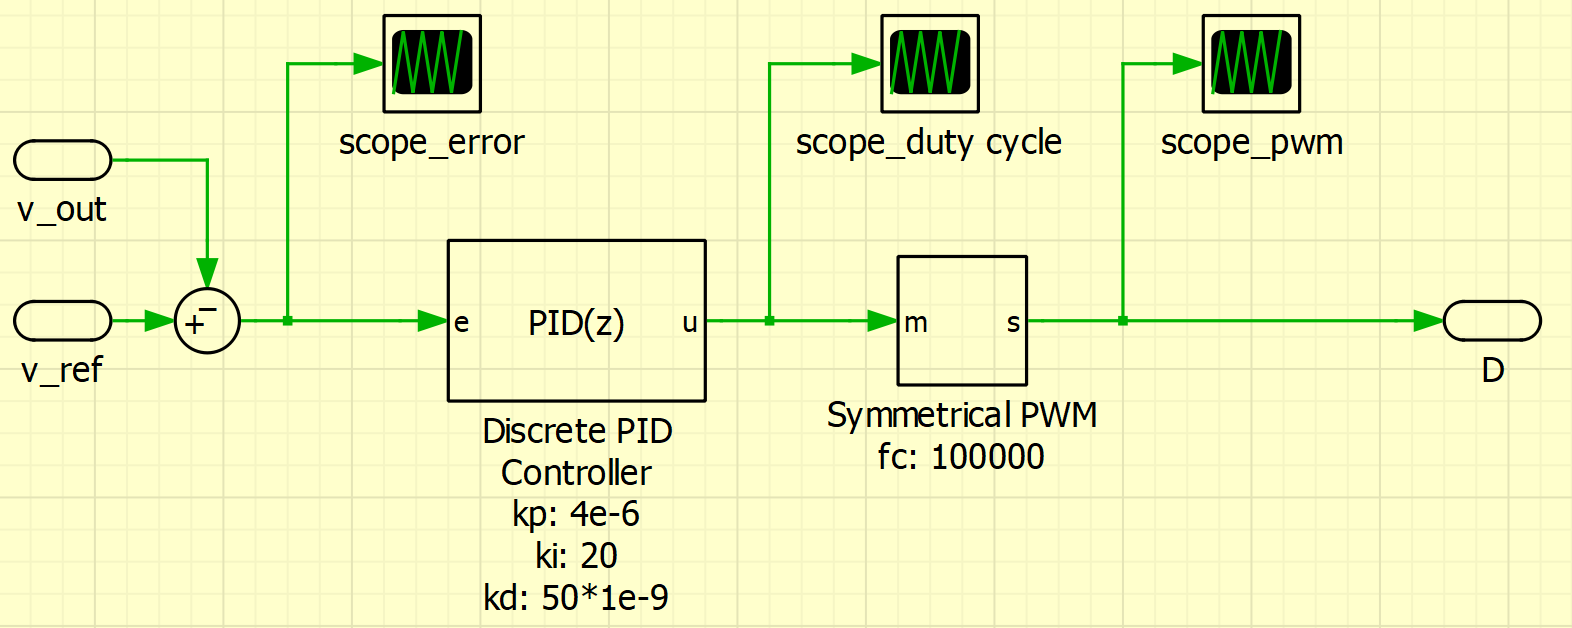
\includegraphics[width=\textwidth]{img/PLECS_PID_Duty_Cycle_control.png}
        \caption{PLECS model of the PID\_Duty\_Cycle\_control subsystem}
        \label{fig:PLECS_PID}
    \end{subfigure}
    \hfill
    \begin{subfigure}[b]{0.40\textwidth}
        \centering
        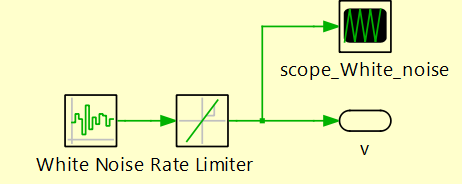
\includegraphics[width=\textwidth]{img/PLECS_noise.png}
        \caption{PLECS model of the noise subsystem}
        \label{fig:PLECS_noise}
    \end{subfigure}
    \caption{PLECS model subsystems}
    \label{fig:PLECS_subsystems}
\end{figure}

\begin{figure}[htbp]
    \centering
    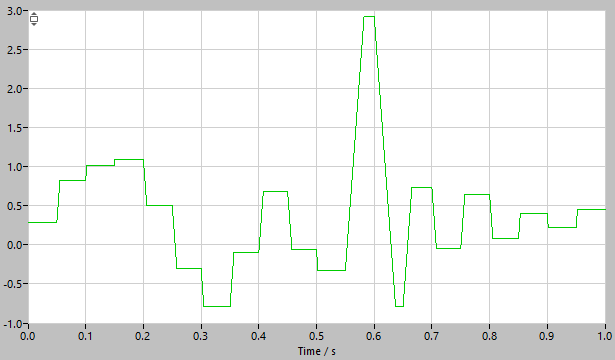
\includegraphics[width=0.8\textwidth]{img/noise.png}
    \caption{White noise with a standard deviation of \qty{1}{\volt} and a sample time of \qty{50}{\milli\second}}
    \label{fig:noise}
\end{figure}

The control of the converter was tested under the following conditions and compared to the behaviour of the converter with a fixed duty cycle:
\begin{itemize}
    \item noise on the input voltage (white noise with a standard deviation of \qty{1}{\volt} and a sample time of \qty{50}{\milli\second} as seen in \autoref{fig:noise})
    \item a load step from \qty{5}{\ohm} to \qty{10}{\ohm} at \qty{0.5}{\second}
    \item startup behaviour
\end{itemize}


% EOF
    % !TEX TS-program = pdflatex
% !TEX encoding = UTF-8 Unicode
% !TEX root = ../main.tex
% !TEX spellcheck = en-US
% ****************************************************************************************
% File: results.tex
% Author: Jakob Spindler
% Date: 2024-10-16
% ****************************************************************************************
\chapter{Results}
\label{chapter:results}
\blindtext




% EOF
    % !TEX TS-program = pdflatex
% !TEX encoding = UTF-8 Unicode
% !TEX root = ../main.tex
% !TEX spellcheck = en-US
% ****************************************************************************************
% File: discussion.tex
% Author: Jakob Spindler
% Date: 2024-10-16
% ****************************************************************************************
\chapter{Discussion}
\label{chapter:discussion}
The uncontrolled converter shows a significant overshoot and oscillation before settling to the working point at startup. The controlled converter shows a much smoother startup behaviour, but the settling time is longer than for the uncontrolled converter as shown in \autoref{fig:comparison_startup}.

The load-jump behaviour of the controlled converter still shows a spike at the load-jump, but quickly settles to the working point as can be seen in \autoref{fig:comparison_load_jump}, whereas the uncontrolled converter delivers a higher unwanted constant ouput voltage after the jump.

The input noise feedthrough of the controlled converter is significantly reduced, although not completely eliminated, compared to the uncontrolled converter as can be seen in \autoref{fig:comparison_input_noise_feedthrough}.

Overall, the behavioural characteristics of the converter have improved with the addition of the \Gls{acr:pid}-Controller.

% EOF

	\pagenumbering{Roman}
	\setcounter{page}{\value{romanpagecount}}
	\stepcounter{page}
	\printbibliography[heading=bibintoc] % This will add the bibliography to the table of contents
    
	%\addcontentsline{toc}{chapter}{\bibname}
	\listoffigures
	\addcontentsline{toc}{chapter}{\listfigurename}
	\listoftables
	\addcontentsline{toc}{chapter}{\listtablename}
	
 
	\clearpage
	\printglossary[type=\acronymtype] % input files created by makeindex
	\printglossary[type=symbolslist,style=symbolsliststyle] % input files created by makeindex

	\appendix
	% !TEX TS-program = pdflatex
% !TEX encoding = UTF-8 Unicode
% !TEX root = ../main.tex
% !TEX spellcheck = en-US
% ****************************************************************************************
% File: appendix.tex
% Author: Jakob Spindler
% Date: 2024-10-16
% ****************************************************************************************
\chapter{Appendix}
\label{chapter:Appendix}



\end{document}
% EOF